\section{Generalizing the \il{put} and \il{get} operations}\label{s:lvars-generalizing}

The determinism result for $\lambdaLVar$ shows that adding LVars (with
their accompanying @new@/@put@/@get@ operations) to an existing
deterministic parallel language (the $\lambda$-calculus) preserves
determinism.  But it is not the case that the @put@ and @get@
operations are \emph{the most general} determinism-preserving
operations on LVars.  In this section, I consider some alternative
semantics for @put@ and @get@ that generalize their behavior while
retaining the determinism of the model.

\subsection{Generalizing from least-upper-bound writes to inflationary, commutative writes}\label{subsection:lvars-generalizing-from-least-upper-bound-writes}

In the LVars model as presented in this chapter so far, the only way
for the state of an LVar to evolve over time is through a series of
least-upper-bound updates resulting from @put@ operations.
Unfortunately, this way of updating an LVar provides no efficient way
to model, for instance, an atomically incremented counter that
occupies one memory location.  Consider an LVar based on the lattice
of Figure~\ref{f:lvars-example-lattices}(c).  Under the
least-upper-bound semantics of @put@, if two independent writes each
take the LVar's contents from, say, $1$ to $2$, then after both
writes, its contents will be $2$, because @put@ takes the maximum of
the previous value and the current value.  Although this semantics is
deterministic, it is not the desired semantics for every application.
Instead, we might want each write to \emph{increment} the contents of
the LVar by one, resulting in $3$.

To support this alternative semantics in the LVars model, we
generalize the model as follows.  For an LVar with lattice $(D,
\userleq, \bot, \top)$, we can define a set of @update@ operations
$\UPDATE_i : D \rightarrow D$, which must meet the following two
conditions:
\begin{itemize}
\item $\forall d, i.     \;\; d \userleq \UPDATE_i(d) $
\item $\forall d, i, j.  \;\; \UPDATE_i(\UPDATE_j(d)) = \UPDATE_j(\UPDATE_i(d)) $
\end{itemize}
The first of these conditions says that an @update@ operation is
inflationary with respect to $\userleq$.  The second condition says
that @update@ operations commute with each other.  In fact, the @put@
operation meets the above two conditions, and therefore can be viewed
as a special case of @update@ that, in addition to being inflationary
and commutative, also happens to compute a least upper bound.

However, when generalizing LVars to support @update@, we must keep in
mind that least-upper-bound @put@ operations do not necessarily mix
with arbitrary @update@ operations on the same LVar.  For example,
consider a set of @update@ operations $\{\UPDATE_{(+1)},
\UPDATE_{(+2)}, \dots \}$ for atomically incrementing a counter
represented by a natural number LVar, with a lattice ordered by the
usual $\leq$ on natural numbers.  The $\UPDATE_{(+1)}$ operation
increments the counter by one, $\UPDATE_{(+2)}$ increments it by two,
and so on.  It is easy to see that these operations commute.  However,
a @put@ of $4$ and a $\UPDATE_{(+1)}$ do not commute: if we start with
an initial state of $0$ and the @put@ occurs first, then the state of
the LVar changes to $4$ since $\max(0, 4) = 4$, and the subsequent
$\UPDATE_{(+1)}$ updates it to $5$.  But if the $\UPDATE_{(+1)}$
happens first, then the final state of the LVar will be $\max(1, 4) =
4$.  Furthermore, multiple distinct families of @update@ functions
only commute among themselves and cannot be combined.

In practice, the author of a particular LVar data structure must
choose which @update@ operations that data structure should provide,
and it is the data structure author's responsibiity to ensure that
they commute.  For example, the LVish Haskell library (which I discuss
in Chapter~\ref{ch:lvish}) provides a set data structure,
@Data.LVar.Set@, that supports only @put@, whereas the counter data
structure @Data.LVar.Counter@ supports only @update@; an attempt to
call @put@ on a @Counter@ would be ruled out by the type system.
However, \emph{composing} LVars that support different families of
@update@ operations is fine.  For example, an LVar could represent a
monotonically growing collection (which supports @put@) of counter
LVars, where each counter is itself monotonically increasing and
supports only @update@.  Indeed, the PhyBin case study described in
Section~\ref{s:lvish-phybin} uses just such a collection of counters.

The determinism of $\lambdaLVar$ relies on the fact that the states of
all LVars evolve monotonically with respect to their lattices, and
that the least upper bound operation is commutative and therefore the
order in which @put@s occur does not matter.  Together, these
properties suffice to ensure that the threshold reads made by @get@
operations are deterministic. The rest of a $\lambdaLVar$ program is
purely functional, and its behavior is, in fact, a pure function of
these @get@ observations.  Since a given family of @update@ operations
is also commutative and inflationary with respect to the lattice of
the LVar they operate on, they preserve determinism.

In Chapter~\ref{ch:quasi}, in addition to extending the LVars model to
support the new features of \emph{freezing} and \emph{event handlers},
I generalize the @put@ operation to @update@.  The resulting
generalized language definition is therefore parameterized not only by
an application-specific lattice, but also by an application-specific
family of commutative and inflationary @update@ operations.

\lk{The Chapter~\ref{ch:quasi} $\lambdaLVish$ result is
  quasi-determinism, not determinism.  So, if I really wanted to be
  serious about showing that \il{update} is deterministic and not
  merely quasi-deterministic, I would do this more modularly: I would
  actually present another version of the $\lambdaLVar$ language here,
  with \il{put} replaced with \il{update}, and then re-do the
  determinism proof for it, instead of just lumping it into the
  quasi-determinism result in the next chapter.  If I did that,
  though, then this section would be big enough to justify being its
  own chapter.  I'm going to just appeal to people's common sense that
  the quasi-determinism in $\lambdaLVish$ comes from freezing, not
  from \il{update}.  I hope that this is OK!}

\subsection{A more general formulation of threshold sets}\label{subsection:lvars-a-more-general-formulation-of-threshold-sets}

Certain deterministic computations are difficult to express using the
definition of threshold sets presented in
Section~\ref{subsection:lvars-communication-primitives}.  For
instance, consider an LVar that stores the result of a parallel
logical ``and'' operation on two Boolean inputs.  I'll call this data
structure an $\mathrm{AndLV}$, and its two inputs the \emph{left} and
\emph{right} inputs, respectively.

We can represent the states an $\mathrm{AndLV}$ can take on as pairs
$(x, y)$, where each of $x$ and $y$ are \il{T}, \il{F}, or \il{Bot}.
The $\andlv{Bot}{Bot}$ state is the state in which no input has yet
been received, and so it is the least element in the lattice of states
that our $\mathrm{AndLV}$ can take on, shown in
Figure~\ref{f:lvars-parallel-and}.  An additional state, \il{Top}, is
the greatest element of the lattice; it represents the situation in
which an error has occurred---if, for instance, one of the inputs
writes \il{T} and then later changes its mind to \il{F}.

\begin{figure}
\begin{center}
  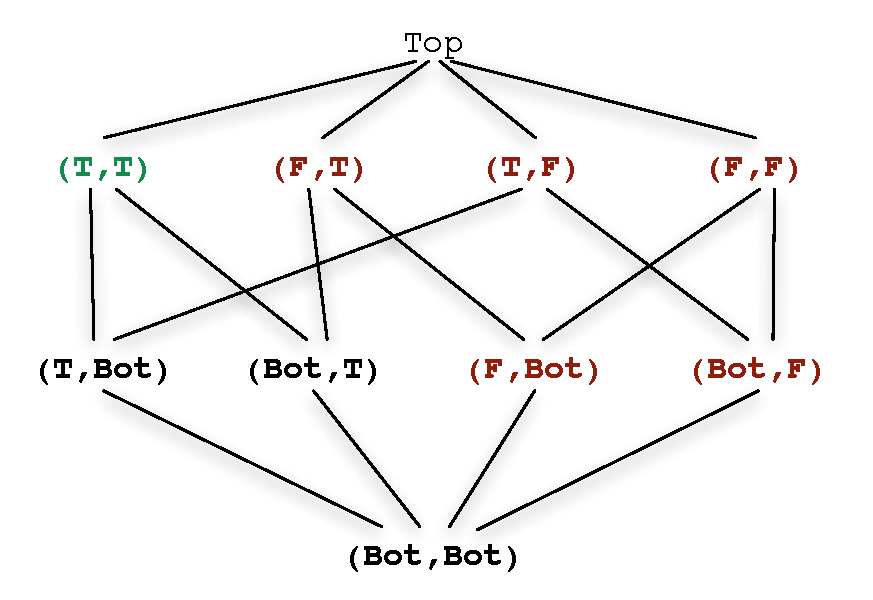
\includegraphics[width=3in]{chapter2/figures/lvars-parallel-and.pdf}
\end{center}
  \caption{Lattice of states that an $\mathrm{AndLV}$ can take on.
    The five red states in the lattice correspond to a false result,
    and the one green state corresponds to a true one.}
  \label{f:lvars-parallel-and}
\end{figure}

The lattice induces a lub operation on pairs of states; for instance,
the lub of $\andlv{T}{Bot}$ and $\andlv{Bot}{F}$ is $\andlv{T}{F}$,
and the lub of $\andlv{T}{Bot}$ and $\andlv{F}{Bot}$ is \il{Top} since
the overlapping \il{T} and \il{F} values conflict.  As usual for
LVars, the @put@ operation updates the $\mathrm{AndLV}$'s state to the
lub of the incoming state and the current state.

We are interested in learning whether the result of our parallel
``and'' computation is ``true'' or ``false''.  Let's consider what
observations it is possible to make of an $\mathrm{AndLV}$ under our
existing definition of threshold reads.  The states $\andlv{T}{T}$,
$\andlv{T}{F}$, $\andlv{F}{T}$, and $\andlv{F}{F}$ are all pairwise
incompatible with one another, and so $\setof{ \andlv{T}{T},
  \andlv{T}{F}, \andlv{F}{T}, \andlv{F}{F} }$---that is, the set of
states in which both the left and right inputs have arrived---is a
legal threshold set argument to @get@.  The trouble with this
threshold read is that it does not allow us to get \emph{early
  answers} from the computation.  It would be preferable to have a
@get@ operation that would ``short circuit'' and unblock immediately
if a single input of, say, $\andlv{F}{Bot}$ or $\andlv{Bot}{F}$ was
written, since no later write could change the fact that the result of
the whole computation would be ``false''.\footnote{Actually, this is
  not quite true: a write of $\andlv{F}{Bot}$ followed by a write of
  $\andlv{T}{Bot}$ would lead to a result of \il{Top}, and to the
  program stepping to the $\error$ state, which is certainly different
  from a result of ``false''.  But, even if a write of
  $\andlv{T}{Bot}$ is due to come along sooner or later to take the
  state of the $\mathrm{AndLV}$ to \il{Top} and thus raise $\error$,
  it should still be fine for the \il{get} operation to allow
  ``short-circuit'' unblocking, because the result of the \il{get}
  operation does not count as observable under our definition of
  observable determinism (as discussed in
  Section~\ref{subsection:lvars-errors-and-observable-determinism}).}
Unfortunately, we cannot include $\andlv{F}{Bot}$ or $\andlv{Bot}{F}$
in our threshold set, because the resulting threshold set would no
longer be pairwise incompatible, and therefore would compromise
determinism.

In order to get short-circuiting behavior from an $\mathrm{AndLV}$
without compromising determinism, we need to make a slight
generalization to how threshold sets and threshold reads work.  In the
new formulation, we divide up threshold sets into subsets that we call
\emph{activation sets}, each consisting of \emph{activation states}.
In the case of the observation we want to make of our
$\mathrm{AndLV}$, one of those activation sets is the set of states
that the data structure might be in when a state containing at least
one \il{F} value has been written---that is, the set $\setof{
  \andlv{F}{Bot}, \andlv{Bot}{F}, \andlv{F}{T}, \andlv{T}{F},
  \andlv{F}{F} }$.  When we reach a point in the lattice that is at or
above any of those states, we know that the result will be ``false''.
The other activation set is the singleton set $\setof{ \andlv{T}{T}
}$, since we have to wait until we reach the state $\andlv{T}{T}$ to
know that the result is ``true''; a state like $\andlv{T}{Bot}$ does
not appear in any of our activation sets.

We can now redefine ``threshold set'' to mean \emph{a set of
  activation sets}.  Under this definition, the entire threshold set
that we would use to observe the contents of our $\mathrm{AndLV}$ is:
\[
\setof{
  \setof{ \andlv{F}{Bot}, \andlv{Bot}{F}, \andlv{F}{T}, \andlv{T}{F}, \andlv{F}{F} },
  \setof{ \andlv{T}{T} }
}
\]
We redefine the semantics of @get@ as follows: if an LVar's state
reaches (or surpasses) any state or states in a particular activation
set in the threshold set, @get@ returns \emph{that entire activation
  set}, regardless of which of its activation states was reached. If
no state in any activation set in the threshold set has yet been
reached, the @get@ operation will block.  In the case of our
$\mathrm{AndLV}$, as soon as either input writes a state containing an
\il{F}, our @get@ will unblock and return the first activation set,
that is, $\setof{ \andlv{F}{Bot}, \andlv{Bot}{F}, \andlv{F}{T},
  \andlv{T}{F}, \andlv{F}{F} }$.  Hence $\mathrm{AndLV}$ has the
expected ``short-circuit'' behavior and does not have to wait for a
second input if the first input contains an \il{F}.  If, on the other
hand, the inputs are $\andlv{T}{Bot}$ and $\andlv{Bot}{T}$, the @get@
will unblock and return $\setof{ \andlv{T}{T} }$.

In a real implementation, of course, the value returned from the @get@
could be more meaningful to the client---for instance, a Haskell
implementation could return \il{False} instead of returning the actual
activation set that corresponds to ``false''.  However, the
translation from $\setof{ \andlv{F}{Bot}, \andlv{Bot}{F},
  \andlv{F}{T}, \andlv{T}{F}, \andlv{F}{F} }$ to \il{False} could just
as easily take place on the client side.  In either case, the
activation set returned from the threshold read is the same regardless
of \emph{which} of its activation states caused the read to unblock,
and it is impossible for the client to tell whether the actual state
of the lattice is, say, $\andlv{T}{F}$, $\andlv{F}{F}$, or some other
state containing \il{F}.

As part of this activation-set-based formulation of threshold sets, we
need to adjust our criterion for pairwise incompatibility of threshold
sets.  Recall that the purpose of the pairwise incompatibility
requirement (see
Section~\ref{subsection:lvars-communication-primitives}) was to ensure
that a threshold read would return a unique result.  We need to
generalize this requirement, since although more than one element
\emph{in the same activation set} might be reached or surpassed by a
given write to an LVar, it is still the case that writes should only
unblock a \emph{unique} activation set in the threshold set.  The
pairwise incompatibility requirement then becomes that elements in an
activation set must be \emph{pairwise incompatible} with elements in
every other activation set.  That is, for all distinct activation sets
$Q$ and $R$ in a given threshold set:
\[
\forall q \in Q.~\forall r \in R.~q \sqcup r = \top
\]
In our $\mathrm{AndLV}$ example, there are two distinct activation
sets, so if we let $Q = \setof{ \andlv{T}{T} }$ and $R = \setof{
  \andlv{F}{Bot}, \andlv{Bot}{F}, \andlv{F}{T}, \andlv{T}{F},
  \andlv{F}{F} }$, the least upper bound of $\andlv{T}{T}$ and $r$
must be \il{Top}, where $r$ is any element of $R$.  We can easily
verify that this is the case.  Furthermore, since the lattice of
states that an $\mathrm{AndLV}$ can take on is finite, the join
function can be verified to compute a least upper bound.

To illustrate why we need pairwise incompatibility to be defined this
way, consider the following (illegal) ``threshold set'' that does not
meet the pairwise incompatibility criterion:
\[
\setof{
\setof{ \andlv{F}{Bot}, \andlv{Bot}{F} },
\setof{ \andlv{T}{Bot}, \andlv{Bot}{T} }
}
\]
A threshold read corresponding to this so-called threshold set will
unblock and return $\setof{ \andlv{F}{Bot}, \andlv{Bot}{F} }$ as soon
as a state containing an \il{F} is reached, and $\setof{
  \andlv{T}{Bot}, \andlv{Bot}{T} }$ as soon as a state containing a
\il{T} is reached.  If, for instance, the left input writes
$\andlv{F}{Bot}$ and the right input writes $\andlv{Bot}{T}$, and
these writes occur in arbitrary order, the threshold read will return
a nondeterministic result, depending on the order of the two writes.
But, with the properly pairwise-incompatible threshold set above, the
threshold read will block until the write of $\andlv{F}{Bot}$ arrives,
and then will deterministically return the ``false'' activation set,
regardless of whether the write of $\andlv{Bot}{T}$ has arrived yet.
Hence ``short-circuit'' evaluation is possible.

Finally, we can mechanically translate the old way of specifying
threshold sets into activation-set-based threshold sets and retain the
old semantics (and therefore the new way of specifying threshold sets
generalizes the old way).  In the translation, every member of the old
threshold set simply becomes a singleton activation set.  For example,
if we wanted a \emph{non}-short-circuiting threshold read of our
$\mathrm{AndLV}$ under the activation-set-based semantics, our
threshold set would simply be
\[
\setof{
  \setof{ \andlv{T}{T} },
  \setof{ \andlv{T}{F} },
  \setof{ \andlv{F}{T} },
  \setof{ \andlv{F}{F} }
},
\]
which is a legal threshold set under the activation-set-based
semantics, but has the same behavior as the old, non-short-circuiting
version.

I use the activation-set-based formulation of threshold sets in
Chapter~\ref{ch:distributed}, where I bring threshold reads to the
setting of replicated, distributed data structures.  I prove that
activation-set-based threshold queries of distributed data structures
behave deterministically (according to a definition of determinism
that is particular to the distributed setting; see
Chapter~\ref{ch:distributed} for more details).

\lk{There's nothing about activation-set-based threshold sets that
  make them more amenable to the distributed setting; I just happened
  to do it that way because, hey, no reason not to do the more general
  thing.  Maybe I should explain that here?}

\subsection{Generalizing from threshold sets to threshold functions}\label{subsection:lvars-generalizing-from-threshold-sets-to-threshold-functions}

The previous section's generalization to activation-set-based
threshold sets prompts us to ask: are further generalizations possible
while retaining determinism?  The answer is \emph{yes}: both the
original way of specifying threshold sets and the more general,
activation-set-based formulation of them can be described by
\emph{threshold functions}.  A threshold function is a partial
function that takes a lattice element as its argument and is undefined
for all inputs that are not at or above a given element in the lattice
(which I will call its \emph{threshold point}), and \emph{constant}
for all inputs that \emph{are} at or above its threshold point.  (Note
that ``not at or above'' is more general than ``below'': a threshold
function is undefined for inputs that are neither above nor below its
threshold point.)

Threshold functions capture the semantics of both the original
style of threshold sets, and the activation-set-based style:
\begin{itemize}
\item In the original style of threshold sets, every element $d$ of a
  threshold set can be described by a threshold function that has $d$
  as its threshold point and returns $d$ for all inputs at or above
  that point.
\item In the activation-set-based style of threshold sets, every
  element $d$ of an activation set $Q$ can be described by a threshold
  function that has $d$ as its threshold point and returns $Q$ for all
  inputs at or above that point.
\end{itemize}
In both cases, inputs for which the threshold functions are undefined
correspond to situations in which the threshold read blocks.

Seen from this point of view, it becomes clear that the key insight in
generalizing from the original style of threshold sets to the
activation-set-based style of threshold sets is that, for inputs for
which a threshold function is defined, its return value need not be
its threshold point. The activation set $Q$ is a particularly useful
return value, but \emph{any} constant return value will suffice.

\lk{By itself, this is kinda unconvincing; what I should really do is,
  at the same time I'm adding generalized \il{update} to
  $\lambdaLVish$ in the next chapter, also add a generalized version
  of \il{get} based on threshold functions.  I think it would look
  something like this: the language has to be parameterized by some
  set $F$ of threshold functions $f_i$.  Then, if someone calls
  $\getexp{l}{\setof{f_1, f_2, \dots}}$, it means that they want to
  get the result of threshold function $f_1$ if $l$ is at or above
  $f_1$'s threshold point; the result of threshold function $f_2$ if
  $l$ is at or above $f_2$'s threshold point, and so on.  In order for
  this to be deterministic, we still need the notion of pairwise
  incompatibility: we need all the \emph{threshold points} of
  threshold functions in a particular call to \il{get} to have $\top$
  as their lub.  Something like that, anyway.  Even though this is
  more general, I'm not sure it is really an improvement to change the
  semantics in this way, because it's arguably even more annoying to
  reason about than threshold sets...}
